% This work is licensed under
% http://creativecommon.org/licenses/by/3.0/
\section{Examples of dynamic-routing mobility in non-hierarchical layers}
\label{sec:sec4}

Dynamic-routing mobility is often used in LANs, which have smaller
scopes and can function without a hierarchical name space.  
%
% JEN: Pamela, check this
%
These LANs handle mobility naturally as part of the normal routing
function, since end-points retain their addresses as they move and
routing does not rely on location-dependent addressing.

\subsection{Wired Ethernet LANs}

An Ethernet LAN is a single layer.
Its member processes are the Ethernet representatives of hosts (endpoints)
and switches (routers),
and its names are MAC addresses.
It has no pre-attachment requirements or configuration for hosts,
which makes it ``plug and play.''

The LAN offers both broadcast and point-to-point services to
higher layers.
In this brief section we do not consider these communication services
further, so
there will be no discussion of the layer's sessions or locations.
Also, for simplicity, we will not extend the modeling into lower levels,
so links in the Ethernet layer are primitives.

An Ethernet layer has two kinds of links.
There are point-to-point links between 
switches, each of which is basically a wire
between two machines.
There are also shared media or buses.
A bus delivers each message
to every machine on the bus, and is used to connect a switch to a
set of hosts.
Either kind of link
can be identified at each switch that
uses it by the port on the switch's machine to which it is attached.

The inter-switch links of the layer must form a bidirectional
spanning tree (see Figure~\ref{fig:ethlinks}). 
Otherwise, when flooding is used (see below), 
the network could be overwhelmed by
messages traveling on cycles.
There are usually more physical links than needed for the spanning tree,
but the extras
can only be used when other links fail and the spanning tree
is recomputed.

\begin{figure}
\centering
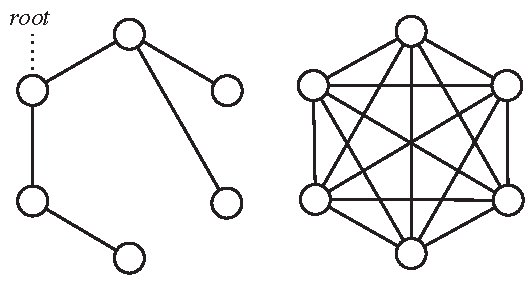
\includegraphics[scale=1.00]{figures/ethlinks.pdf}
\caption{Inter-switch links of an Ethernet LAN layer (left) and an overlay
layer (right).
The Ethernet links are physical, while the overlay links are virtual.}
\label{fig:ethlinks}
\end{figure}

Each switch has a forwarding table containing {\it (MAC address, port)}
pairs.
The port identifies the link on which the switch should forward messages
destined for the MAC address.  
Each switch's table is sparse and is populated lazily by a routing
algorithm called ``MAC learning.''
Upon receiving a message with a source MAC 
address that is not in its forwarding
table, the switch adds to its table the MAC address and the link
on which the message was received.

The forwarding algorithm of a switch is similarly simple.
Upon receiving a message not destined for itself, the switch looks for the
destination MAC address in its own forwarding table.
If it finds an entry, it forwards the message on the designated link.
If it does not find an entry, it ``floods'' by forwarding the message
on every link except the one on which it was received.

These mechanisms implement dynamic-routing mobility as an
aspect of normal operation rather than as a special case.
When a host moves within the layer, it changes the link through which
it is attached to the layer.
As soon as it sends messages, new routes to it begin to propagate through
the layer.
Obsolete forwarding-table entries
are removed when their time-to-live expires.
Missing table entries are handled by flooding.
Note that an entry might also be removed from a forwarding table because
the table is full and space for a newer entry is needed.

\subsection{Ethernet overlays}

Several recent
designs~\cite{seattle,vl2,nvp} avoid flooding by forming
an overlay topology that interconnects all of the edge switches, as
shown on the right side of Figure~\ref{fig:ethlinks}.  While the
inter-switch links of an Ethernet are physical and form a spanning
tree, the inter-switch links of an overlay network are virtual and
fully connect the switches.  

The virtual links are communication services implemented by a second,
lower layer.  For example, Figure~\ref{fig:seattle} shows the path of
a message from host {\it Hv} to host {\it Hz} (the lower-case letters
stand for their MAC addresses).  On each hop, the path is labeled with
the source name above and the destination name below.  The virtual hop
between switches {\it Sw} and {\it Sy} in the overlay layer is
implemented in the underlay, where the message is encapsulated in a
message with source {\it w} and destination {\it y}.

How are the virtual links in the overlay implemented by the underlay?
The members of the underlay layer are the switches
only, not the hosts.  Each switch's name is the MAC address of its
machine, just as in the overlay, so there is no need for a 
{\it locations} state component to map one name to another.  
The members of the underlay are stable and
stationary.  Routing is static except for failures, and the forwarding
tables are fully populated.  Because there is no flooding, there is no
need to restrict the links to a spanning tree, and all of the physical
links between switches can be fully utilized.  
The underlay can run an efficient routing protocol, such as a link-state
protocol, to compute a shortest path from one edge switch to
another.

\begin{figure}
\centering
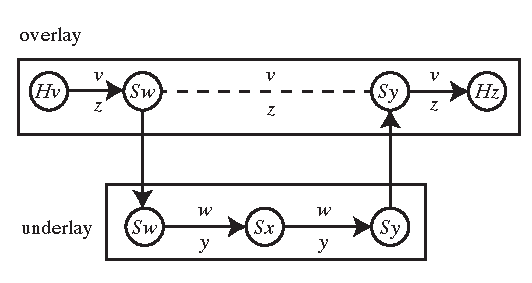
\includegraphics[scale=1.00]{figures/seattle.pdf}
\caption{The path of a message through two layers and three
switches.}
\label{fig:seattle}
\end{figure}

Routing in the overlay is unusual compared to routing in general,
because every edge switch is directly linked to every other edge switch.
This means that an inter-switch route to a host
can be identified simply by the
MAC address of the host's edge switch, and is exactly the same
no matter which switch needs the route!
Thus inter-switch routing is a mapping that is {\it global}
within the layer.
%
% JEN: Pamela, check this
%
Note that, despite the use of a single global directory, the mapping
performed is indeed part of \emph{routing} within the layer (i.e., the
{\it routes} mapping), \emph{not} a {\it locations} mapping between
two layers.  The underlay layer in Figure~\ref{fig:seattle} exists to
make the \emph{routing} between the edge switches more scalable, not
to implement the \emph{link} between the two end-points.

As with Ethernet LANs, each switch has a routing table that is
populated lazily ({\it e.g.}, through MAC learning).
The difference lies in what happens when a switch needs a route to
an unknown destination.
Rather than flooding, it looks the route up in a global routing
directory.

When a host moves, the directory is
updated with the new route to the host.  The exact update mechanism
differs from one overlay design to another, depending on whether
mobility is planned ({\it e.g.,} 
virtual-machine migration in a data center)
or unplanned ({\it e.g.,} a mobile device moving within a campus).  In a
data center, a central controller that triggers virtual-machine
migration can also update the directory with the new
route~\cite{vl2,nvp}.  If the directory cannot be informed in advance
that a host is moving, the new local switch can learn that a new
device has connected and subsequently update the
directory~\cite{seattle}.

The routing directory in an overlay is an important part of its design, 
and may have
many features to make both queries and updates fast and efficient.
Different designs have different directory structures.  VL2~\cite{vl2}
and NVP~\cite{nvp} run a centralized directory on a collection of
server machines.  In these designs, if the ingress switch {\it Sw}
does not know the route for host {\it Hz}, {\it Sw} queries a
directory server to learn the route {\it Sy}.  In contrast,
SEATTLE~\cite{seattle} implements the directory as a ``one-hop
Distributed Hash Table''~\cite{gupta} running directly on the
switches.  
If the ingress switch {\it Sw} does not know the route for
host {\it Hz}, {\it Sw} computes the hash of the {\it Hz}'s MAC
address and forwards the message over a single overlay link to the
switch responsible for this hashed value.  This switch, in turn,
forwards the message to {\it Hz}'s local switch {\it Sy} and informs
switch {\it Sw} of the route for {\it Hz} so that future messages flow
directly from {\it Sw} to {\it Sy}.

To improve the speed of mobile handoff, the ingress switch {\it Sw}
can receive an update when a host moves to a new location.  To perform
these updates, the directory could maintain information about all
ingress switches that recently queried the directory for a route to
{\it Hz}.  However, this can require the directory to maintain a large
amount of state.  Instead, when a host moves, the directory can update
the mobile host's old local switch.  Upon receiving a message for the
mobile host, the old local switch can both forward the message to the
mobile host and send an immediate notification about the new route to
the sending switch~\cite{seattle}.  This reactive invalidation of
stale routes obviates the need for the directory to maintain
information about which ingress switches sent queries for {\it Hz},
while still ensuring rapid invalidation of stale routes.

In addition to SEATTLE, VL2, and NVP, several other designs adopt
certain aspects of the overlay solution.  
The early work on
Rbridges~\cite{rbridges}, and the resulting TRILL~\cite{rfc5556}
standard at the IETF, also forms an Ethernet overlay with
shortest-path routing in the underlay.  
However, instead of having an
explicit directory service, TRILL relies on flooding to reach hosts
with unknown routes.  
Rather than flooding on all normal overlay links, TRILL floods
on a special multicast link in the overlay.
This special link is implemented in the underlay by a multicast tree
formed on the underlay topology.

Like VL2 and NVP, the PortLand~\cite{portland} design
has a set of directory servers that allow ingress switches to learn
the route to a destination host.  Instead of encapsulating a message,
PortLand assigns each edge switch a block of host ``pseudo-MAC
addresses'' and rewrites the host MAC addresses at the edge.  To
enable the use of hierarchical pseudo-MAC addresses, PortLand is
restricted to the tree topologies common in data-center networks.
Table~\ref{tab:overlays} summarizes the structural characteristics
of all five designs.

\begin{table}
\begin{center}
\begin{tabular}{|l|l|l|} \hline
\multicolumn{1}{|c|}{\bf Protocol} &
 \multicolumn{1}{c|}{\bf Routing Directory} &
 \multicolumn{1}{c|}{\bf Encapsulation} \\ \hline
SEATTLE &
 one-hop DHT on the switches &
 simple encapsulation \\
VL2 &
 directory servers &
 simple encapsulation \\
NVP &
  directory servers &
  simple encapsulation\\
Rbridges/TRILL &
  none, flooding on multicast tree &
  simple encapsulation\\
PortLand &
 directory servers &
 none, MAC rewriting\\
\hline 
\end{tabular}
\end{center}
\caption{Ethernet overlay designs for dynamic-routing mobility.}
\label{tab:overlays}
\end{table}

\subsection{Comparative resource costs}
\label{sec:props}

Concerning storage costs, both Ethernet LANs and overlay designs
incur the costs of the
forwarding tables in switches.
These costs are kept moderate by the fact that the tables are sparsely
populated.
Because there is no aggregation of names or table entries, the costs
of densely populated tables would be too great.
In addition to the forwarding tables, the overlay designs incur a storage cost
for the routing directory, which maintains global state for the layer.

Concerning update costs, both approaches incur negligible costs for 
populating forwarding tables lazily through MAC learning.
The biggest update cost is the cost of Ethernet flooding.
The cost of flooding, in terms of bandwidth, grows quadratically with the
size of the network---which makes it a potential scalability problem.
Whether it becomes an actual problem or
or not depends on its frequency, which
depends on both the frequency of moves and the number of correspondents
that a mobile host tends to have.
SEATTLE, VL2, NVP, and PortLand have no flooding cost, though
they do have the additional cost of updating the directory.

Mobility in the overlay designs incurs no path cost.
The path cost of Ethernet mobility is significant, because the spanning
tree (which is necessitated by flooding) forces paths to be longer and
forces some physical links to go unused.

We can measure handoff latency from the instant when the mobile host
re-attaches to the network and informs its local switch (before that
time no mobility mechanism can take effect).
The following scenarios assume that a correspondent switch is sending
a steady stream of messages to a mobile host.
They describe the elapse of time before messages sent by the
correspondent switch (CS) are forwarded to the mobile host at its new
attachment.

The Ethernet scenario:
\begin{enumerate}
\item
The time-to-live of the CS's route to the mobile host expires, if it has
not already.
\item
CS receives the next message from the correspondent host and floods it.
\item
After a round trip to the mobile host, CS learns the new route.
\end{enumerate}
After Step 3, messages sent by CS are forwarded to the mobile host at
its new attachment.

In the directory-based overlay solutions ({\it i.e.,}
SEATTLE, VL2, NVP, and PortLand):
\begin{enumerate}
\item
The directory receives an update of the mobile host's new local switch.
\item
The directory informs the mobile host's old local switch of the new route.
\item
The next message arrives at the mobile host's old local switch, and
is forwarded on the new route.
\item
The mobile host's old switch also informs the CS of the new route.
\end{enumerate}
At Step 3 and after, messages sent by CS are forwarded to the mobile
host at its new attachment.
If Step 1 of the Ethernet scenario takes time, then the handoff latency
of the overlay designs will be smaller than the Ethernet's.

In addition to resource costs,
security and privacy are ever-present concerns.
In Section~\ref{sec:majordifferences} we noted that DRM usually
has minimal security problems because only routers participate
in routing.
Ethernet flooding is an exception to this rule because 
it allows hosts to play a role in routing.
Malicious
hosts can force flooding by filling up the network's forwarding tables.
(This would be accomplished by sending many messages from spoofed
source MAC addresses.)
Severe flooding can cause denial of service.
Also, the
malicious hosts will receive all the flooded packets, which
may contain private information that they wish to see.
